\section{Introducción}

El  particionado  del  espacio  por  estructuras  arbóreas  divide  una  región  en  varias  partes, que pueden ser divididas en otras partes más pequeñas sucesivamente. Para entender los kd-trees es necesario comprender primero cómo funcionan los quadtrees/octrees.Quadtrees y octrees son semejantes, salvo que cuando se trabaja en dos dimensiones se usan quadtrees (cada nodo despliega cuatro hijos) y en tres dimensiones octrees(cada nodo despliega ocho hijos). \\

Un  kd-tree  es un  árbol  binario  en  el  que  cada  división  de  una  región se  parte  en dos regiones disjuntas. Cada una de ellas puede dividirse en dos más pequeñas sucesivamente hasta los  nodos  hoja,donde se  guarda  el  listado  de  los  objetos  que intersecan  con su  región.A diferencia del quadtree la división no tiene por qué generar dos particiones iguales. Para hacer el corte  o  división,  se  utiliza una  recta  (para  dos  dimensiones)  o  un  plano  (para  tres  dimensiones) alineados con los ejes de coordenadas.

\begin{figure}[H]
  \centering
  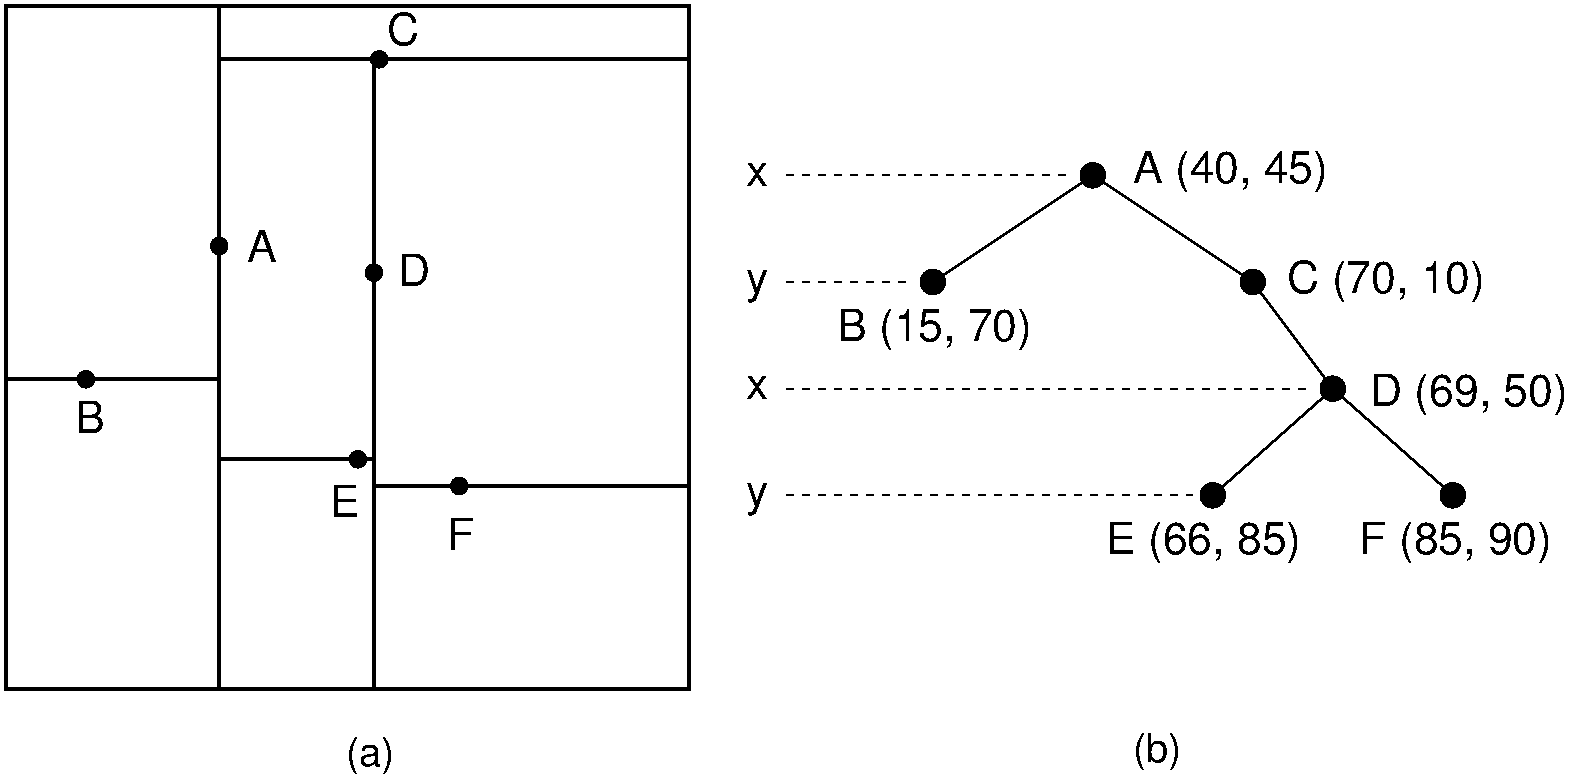
\includegraphics[width=0.8\textwidth]{images/KDtree.png}
  \caption{(a)La descomposición del árbol kd para una región. (b)El árbol kd para la región a}
  \label{fig:act-kdtree}
\end{figure}